%\nocite{0a816f4c}
%%%
For a 1-dimensional ordinary TQFT
\begin{align*}
  Z
  \colon
  \mathbf{Cob}_{1}
  &\to
  \mathbf{Vec}_{K}
\end{align*}
we have a finite-dimensional vector space $Z(S)$ associated to every closed oriented $0$-manifold $S \in \mathrm{ob}_{\mathbf{Cob}_{1}}$. Such a manifold is a finite set of points, where each point has a positive or negative orientation, so that we can consider the manifold as a disjoint union of positive points and of negative points, as there always is an orientation-preserving diffeomorphism\footnote{remember that an orientation-preserving diffeomorphism induces an isomorphism in the cobordism category via the cylinder construction} to such a disjoint union. This means that there are two points (at least up to orientation-preserving diffeomorphism), the positively oriented point $\bullet_{+}$ and the negatively oriented point $\bullet_{-} = \overline{\bullet_{+}}$, that build up all objects in $\mathbf{Cob}_{1}$ by disjoint union. Hence, for $S$ we can write
\begin{align*}
  S
  &\cong
  \bullet_{+}^{\sqcup k}
  \sqcup
  \bullet_{-}^{\sqcup m}
\end{align*}
for some $k,m \in \mathbb{N}$, where the superscript $\sqcup k$ means $k$-fold disjoint union. The TQFT $Z$ assigns a finite-dimensional vector space to each of these points, yet, as $\bullet_{-}$ is a dual object of $\bullet_{+}$ we know that $Z(\bullet_{-})$ is canonically isomorphic to the dual space $V^{\prime}$ of $Z(\bullet_{+}) =: V$. Moreover, as $Z$ is a symmetric monoidal functor, $Z(S)$ is canonically isomorphic\footnote{by the natural isomorphism that is part of the symmetric monoidal functor which we did not make explicit here; we did not make explicit the isomorphism for the unit objects either but both will be tacitly used here for identifications} to
\begin{align*}
  V^{\otimes k}
  \otimes
  (V^{\prime})^{\otimes m}
\end{align*}
where the superscript $\otimes k$ means $k$-fold tensor product. From this we see that $Z$ is determined on objects by only one datum, namely the finite-dimensional vector space associated to the positively oriented\footnote{this is just a matter of convention, as there is certainly no reason to prefer the positive orientation, and we might equivalently choose the negatively oriented point} point.
\\
Now what happens on the level of morphisms? As $Z$ is symmetric monoidal, disjoint unions are basically taken to tensor products on the morphism level, too, so that it suffices to consider connected cobordism classes. A connected smooth compact 1-manifold with boundary is either diffeomorphic to the closed interval $[0,1]$ or to the circle $S^{1}$ but we also have to take orientations and in- and out-boundaries into account. For the circle this does not matter as there are no boundaries and there is an orientation-reversing diffeomorphism for the circle (a reflection), i.e. the circle with the opposite orientation represents the same morphism as with the original orientation. For the closed interval $[0,1]$ there are different cases to consider:
\begin{enumerate}
\item[i)]
The interval $M = [0,1]$ can represent the identity for $\bullet_{+}$ or $\bullet_{-}$, that is $\mathrm{id}_{\bullet_{+}}$ or $\mathrm{id}_{\bullet_{-}}$ as pictured below (remember we depict cobordisms from top down).
\begin{equation*}
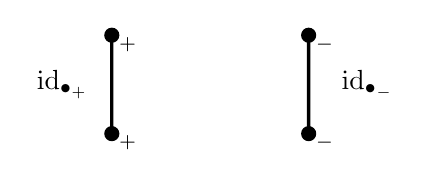
\begin{tikzpicture}[scale=1.25,very thick]
  \filldraw
    (0,0) circle (1.7pt) node[shift={(0.2,-0.12)}] {\scriptsize{$+$}}
    --
    (0,1) circle (1.7pt) node[shift={(0.2,-0.12)}] {\scriptsize{$+$}};
  \filldraw
    (2,0) circle (1.7pt) node[shift={(0.2,-0.12)}] {\scriptsize{$-$}}
    --
    (2,1) circle (1.7pt) node[shift={(0.2,-0.12)}] {\scriptsize{$-$}};
  \draw
    (-0.5,0.5) node[fill=white] {$\mathrm{id}_{\bullet_{+}}$}
    (2.6,0.5) node[fill=white] {$\mathrm{id}_{\bullet_{-}}$};
\end{tikzpicture}
\end{equation*}
Since $Z$ is a functor we find in these cases that $Z([M])$ is just $\mathrm{id}_{V}$ or $\mathrm{id}_{V^{\prime}}$

\item[ii)]
The interval $M = [0,1]$ can represent a cobordism from the empty 0-manifold $\emptyset$ to $\bullet_{+} \sqcup \bullet_{-}$, namely the coevaluation $\mathrm{coev}_{\bullet_{+}}$. Analogously, it can represent the coevaluation $\mathrm{coev}_{\bullet_{-}}$ for $\bullet_{-}$.
\begin{equation*}
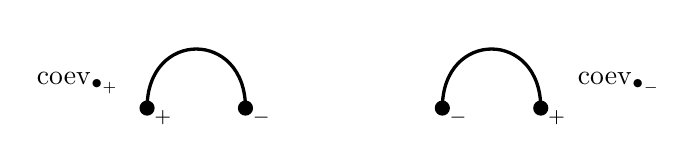
\begin{tikzpicture}[scale=1.25,very thick]
  \filldraw
    (0,0) circle (1.7pt) node[shift={(0.2,-0.12)}] {\scriptsize{$+$}}
    (1,0) circle (1.7pt) node[shift={(0.2,-0.12)}] {\scriptsize{$-$}};
  \draw
    (0,0)
    ..
    controls
    +(0,0.8)
    and
    +(0,0.8)
    ..
    (1,0);
  \filldraw
    (3,0) circle (1.7pt) node[shift={(0.2,-0.12)}] {\scriptsize{$-$}}
    (4,0) circle (1.7pt) node[shift={(0.2,-0.12)}] {\scriptsize{$+$}};
  \draw
    (3,0)
    ..
    controls
    +(0,0.8)
    and
    +(0,0.8)
    ..
    (4,0);
  \draw
    (-0.7,0.25) node[fill=white] {$\mathrm{coev}_{\bullet_{+}}$}
    (4.8,0.25) node[fill=white] {$\mathrm{coev}_{\bullet_{-}}$};
\end{tikzpicture}
\end{equation*}
As $Z$ is monoidal, $Z([M])$ can be identified with the coevaluations for $V$ and $V^{\prime}$ respectively, i.e. for a basis $\lbrace v_{1},\ldots,v_{l} \rbrace$ of $V$ (supposed that the dimension of $V$ is $l \in \mathbb{N}$) and the corresponding dual basis $\lbrace v_{1}^{\prime},\ldots,v_{l}^{\prime} \rbrace$ of $V^{\prime}$ we obtain
\begin{align*}
  \mathrm{coev}_{V}
  \colon
  K
  \to
  V
  \otimes
  V^{\prime}
  ,\qquad
  x
  &\mapsto
  x
  \sum_{i=1}^{l}
  v_{i}
  \otimes
  v_{i}^{\prime}
\end{align*}
or
\begin{align*}
  \mathrm{coev}_{V^{\prime}}
  \colon
  K
  \to
  V^{\prime}
  \otimes
  V
  ,\qquad
  x
  &\mapsto
  x
  \sum_{i=1}^{l}
  v_{i}^{\prime}
  \otimes
  v_{i}
\end{align*}
for $Z([M])$.

\item[iii)]
The interval $M = [0,1]$ can represent a cobordism from $\bullet_{-} \sqcup \bullet_{+}$ to the empty 0-manifold $\emptyset$, namely the evaluation $\mathrm{ev}_{\bullet_{+}}$. Analogously, it can represent the evaluation $\mathrm{ev}_{\bullet_{-}}$ for $\bullet_{-}$.
\begin{equation*}
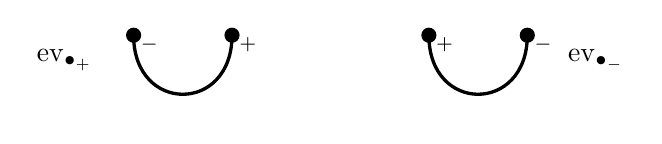
\begin{tikzpicture}[scale=1.25,very thick]
  \filldraw
    (0,0) circle (1.7pt) node[shift={(0.2,-0.12)}] {\scriptsize{$-$}}
    (1,0) circle (1.7pt) node[shift={(0.2,-0.12)}] {\scriptsize{$+$}};
  \draw
    (0,0)
    ..
    controls
    +(0,-0.8)
    and
    +(0,-0.8)
    ..
    (1,0);
  \filldraw
    (3,0) circle (1.7pt) node[shift={(0.2,-0.12)}] {\scriptsize{$+$}}
    (4,0) circle (1.7pt) node[shift={(0.2,-0.12)}] {\scriptsize{$-$}};
  \draw
    (3,0)
    ..
    controls
    +(0,-0.8)
    and
    +(0,-0.8)
    ..
    (4,0);
  \draw
    (-0.7,-0.25) node[fill=white] {$\mathrm{ev}_{\bullet_{+}}$}
    (4.7,-0.25) node[fill=white] {$\mathrm{ev}_{\bullet_{-}}$};
\end{tikzpicture}
\end{equation*}
As $Z$ is monoidal, $Z([M])$ can be identified with the evaluations for $V$ and $V^{\prime}$ respectively, i.e. we obtain
\begin{align*}
  \mathrm{ev}_{V}
  \colon
  V^{\prime}
  \otimes
  V
  \to
  K
  ,\qquad
  v^{\prime}
  \otimes
  v
  &\mapsto
  v^{\prime}(v)
\end{align*}
or
\begin{align*}
  \mathrm{ev}_{V^{\prime}}
  \colon
  V
  \otimes
  V^{\prime}
  \to
  K
  ,\qquad
  v
  \otimes
  v^{\prime}
  &\mapsto
  v^{\prime}(v)
\end{align*}
for $Z([M])$.
\end{enumerate}
Therefore, in any case the morphisms represented by the closed interval $[0,1]$ are determined by the duality properties of $V$. In the case of the circle $S^{1}$ which has empty in- and out-boundary the TQFT $Z$ must determine an element of $K$. But we already know that this must be the dimension $\dim(V)$ of the vector space $V$ since the circle can be understood as a representation of
\begin{align*}
  \mathrm{ev}_{\bullet_{+}}
  \circ
  \mathsf{B}
  \left(
    \bullet_{+}
    ,
    \bullet_{-}
  \right)
  \circ
  \mathrm{coev}_{\bullet_{+}}
\end{align*}
(cf. corollary \ref{cor:dimS1} in chapter \ref{CHAP:ALTCHARPROPS}), where $\mathrm{B}$ is the symmetric braiding of $\mathbf{Cob}_{1}$. Hence we see that $Z$ is entirely determined (at least up to isomorphism) by specifying the finite-dimensional vector space $Z(\bullet_{+}) = V$. And indeed, one can construct a one-dimensional TQFT from every finite dimensional vector space in the above way, so that we basically have a 1-to-1 correspondence between 1-dimensional TQFTs and finite dimensional vector spaces.
\\
This illustrates that even though a priori there are many data to specify for a TQFT, it may be already determined by only a small part of these data - in the 1-dimensional case, for example, by only one datum. Note however that manifolds which need not be specified explicitly may still carry interesting information - in the 1-dimensional case, for example, one obtains the dimension of the vector space which determines the TQFT by considering the circle $S^{1}$ (which, as seen in corollary \ref{cor:dimS1} in chapter \ref{CHAP:ALTCHARPROPS}, can be generalized to higher dimensions).
\\
Now the 1-dimensional TQFTs are the objects of the category
\begin{align*}
  \mathbf{TQFT}_{1}
  &=
  \mathrm{func}^{\otimes,\mathrm{sym}}
  \left(
    \mathbf{Cob}_{1}
    ,
    \mathbf{Vec}_{K}
  \right)
\end{align*}
the morphisms being the monoidal natural transformations, and in fact this category is a groupoid. To cast this example in a nice categorical language we would like to have some algebraic structure that forms a groupoid and captures the structure of finite-dimensional vector spaces in such a way that this groupoid is equivalent to the groupoid of 1-dimensional TQFTs. The natural choice seems to be the category $\mathbf{Finvec}_{K}$ of finite-dimensional vector spaces and linear maps as morphisms. But unfortunately this is not a groupoid since linear maps need not be invertible. Yet, there is an underlying groupoid of this category obtained by discarding all non-invertible linear maps and this is indeed equivalent to $\mathbf{TQFT}_{1}$. But there also is another category in which the inherent duality structure of objects is made a bit more explicit: the category $\mathbf{DP}_{K}$ of dual pairs as described, for example, in \cite{0a816f4c} with the following data
\begin{enumerate}
\item[$\bullet$]
objects are tuples $(V_{1},V_{2},b,d)$ consisting of vector spaces $V_{1},V_{2}$ and two linear maps
\begin{align*}
  b
  \colon
  K
  &\to
  V_{1}
  \otimes
  V_{2}
  ,\qquad
  d
  \colon
  V_{2}
  \otimes
  V_{1}
  \to
  K
\end{align*}
usually called {\glqq}birth{\grqq} and {\glqq}death{\grqq}, which satisfy the conditions (LD1) and (LD2) for dual objects (as vector spaces)

\item[$\bullet$]
morphisms from objects $(V_{1},V_{2},b,d)$ to $(\hat{V}_{1},\hat{V}_{2},\hat{b},\hat{d})$ are pairs $(f_{1},f_{2})$ of linear maps $f_{1} \colon V_{1} \to \hat{V}_{1}$ and $f_{2} \colon V_{2} \to \hat{V}_{2}$ that are subject to the following constraints
\begin{align*}
  (f_{1} \otimes f_{2})
  \circ
  b
  &=
  \hat{b}
  ,\qquad
  d
  =
  \hat{d}
  \circ
  (f_{2} \otimes f_{1})
\end{align*}
\end{enumerate}
Note that the duality conditions for objects enforce the vector spaces in an object of $\mathbf{DP}_{K}$ to be of the same finite dimension. Note further that the conditions for morphisms encode their compatibility with the duality structure and in fact this ensures that they are invertible (this can be seen in a similar way as in the proof of theorem \ref{thm:mntiso} in chapter \ref{CHAP:ALTCHARPROPS}) so that $\mathbf{DP}_{K}$ is a groupoid. Now one can show that the assignment
\begin{align*}
  Z
  &\mapsto
  \left(
    Z(\bullet_{+})
    ,
    Z(\bullet_{-})
    ,
    \mathrm{coev}_{Z(\bullet_{+})}
    ,
    \mathrm{ev}_{Z(\bullet_{+})}
  \right)
\end{align*}
induces a functor that is an equivalence between $\mathbf{TQFT}_{1}$ and $\mathbf{DP}_{K}$.
\\
One can also phrase this example in yet another way, namely by a generators-and-relations approach in terms of free(ly) (generated) symmetric monoidal categories. Given a set $G_{0}$ of objects, a set $G_{1}$ of morphisms and a set $G_{2}$ of relations the morphisms in $G_{1}$ are subject to, one can construct a symmetric monoidal category $\mathbf{F}(G_{0},G_{1},G_{2})$ satisfying a universal property which can basically, but a bit unprecisely, be stated as follows:
\begin{quotation}
For $\mathbf{C}$ a symmetric monoidal category, a symmetric monoidal functor from $\mathbf{F}(G_{0},G_{1},G_{2})$ to $\mathbf{C}$ is determined uniquely up to natural monoidal isomorphism by choosing an object in $\mathrm{ob}_{\mathbf{C}}$ for each element in $G_{0}$ and a morphism in $\mathrm{Mor}_{\mathbf{C}}$ with correct source and target for every element in $G_{1}$ in such a way that the relations in $G_{2}$ are satisfied.
\end{quotation}
This category $\mathbf{F}(G_{0},G_{1},G_{2})$ is consequently unique up to natural monoidal isomorphism and is called the \textit{symmetric monoidal category freely generated by $G_{0},G_{1},G_{2}$}. A nice overview for this construction is given in \cite{0a816f4c}. One can show that $\mathbf{Cob}_{1}$ is freely generated by objects
\begin{align*}
  G_{0}
  &=
  \lbrace
    \bullet_{+}
    ,
    \bullet_{-}
  \rbrace
\end{align*}
morphisms
\begin{align*}
  G_{1}
  &=
  \lbrace
    \mathrm{coev}_{\bullet_{+}}
    ,
    \mathrm{ev}_{\bullet_{+}}
  \rbrace
\end{align*}
and relations $G_{2}$ the duality constraints\footnote{the careful reader may have noticed that apart from $\bullet_{+}$ all other data are determined by duality; for this reason one also says that $\mathbf{Cob}_{1}$ is the \textit{free symmetric monoidal category with duals generated by one object}}. Going through the construction, as is done in \cite{0a816f4c}, one hence obtains precisely the equivalence between $\mathbf{TQFT}_{1}$ and $\mathbf{DP}_{K}$.
